\documentclass[letterpaper]{article} % DO NOT CHANGE THIS
\usepackage[submission]{aaai2027} % DO NOT CHANGE THIS
\usepackage[hyphens]{url} % DO NOT CHANGE THIS
\usepackage{graphicx} % DO NOT CHANGE THIS
\urlstyle{rm} % DO NOT CHANGE THIS
\def\UrlFont{\rm} % DO NOT CHANGE THIS
\usepackage{natbib} % DO NOT CHANGE THIS
\usepackage{caption} % DO NOT CHANGE THIS
\frenchspacing % DO NOT CHANGE THIS
\usepackage{booktabs}
\usepackage{amsmath,amssymb,amsthm,mathtools}

\pdfinfo{
/TemplateVersion (2027.1)
}
\setcounter{secnumdepth}{0}

\newtheorem{theorem}{Theorem}
\newtheorem{proposition}{Proposition}
\newtheorem{lemma}{Lemma}
\newtheorem{corollary}{Corollary}
\newcommand{\E}{\mathbb E}
\newcommand{\Pp}{\mathbb P}
\newcommand{\cA}{\mathcal A}
\newcommand{\cX}{\mathcal X}
\newcommand{\spanop}{\operatorname{span}}
\newcommand{\KL}{D_{\mathrm{KL}}}

\title{Technical Supplement:\\
How Much History Is Enough? Certifying Decision-Relevant Memory in Offline Reinforcement Learning}
\author{Anonymous Submission}
\affiliations{Anonymous submission}

\begin{document}
\maketitle

\section{Notation}

At stage \(h\), \(X_h\) is the full observable history and
\(\phi_{m,h}(X_h)\) is its \(m\)-observation suffix.  The suffix cell is
\(C_{m,h}(z)=\{x:\phi_{m,h}(x)=z\}\).  We use
\(A_h^*(x,a)=V_h^*(x)-Q_h^*(x,a)\),
\[
\eta_{m,h}(z)=\min_{p\in\Delta(\cA_h)}
\max_{x\in C_{m,h}(z)}\E_{a\sim p}A_h^*(x,a),
\]
\(\eta_{m,h}=\max_z\eta_{m,h}(z)\), and
\(G_m=\sum_h\eta_{m,h}\).

\section{Population Proofs}

\begin{lemma}[Monotonicity]
For every stage, \(\eta_{m+1,h}\leq\eta_{m,h}\), and therefore
\(G_{m+1}\leq G_m\).
\end{lemma}
\begin{proof}
Every \((m+1)\)-suffix cell \(C'\) lies inside one \(m\)-suffix cell \(C\).
Let \(p_C\) minimize the objective for \(C\).  Then
\[
\begin{aligned}
\eta(C')
&\leq\max_{x\in C'}\E_{a\sim p_C}A_h^*(x,a)\\
&\leq\max_{x\in C}\E_{a\sim p_C}A_h^*(x,a)=\eta(C).
\end{aligned}
\]
Taking the maximum over refined cells proves the stagewise claim; summing
proves the cumulative claim.
\end{proof}

\begin{theorem}[Exact sufficiency]
For a fixed \(m\), \(G_m=0\) if and only if there exists an \(m\)-suffix
policy that is optimal from every full context at every stage.
\end{theorem}
\begin{proof}
All entries of \(A_h^*\) are nonnegative.  Thus a cell has zero minimax value
if and only if some action distribution \(p_{h,z}\) has zero expected
advantage loss at every context in the cell.  Use these distributions to form
a suffix policy \(\pi\).  At stage \(H\),
\(V_H^\pi(x)=\E_{a\sim p_{H,z}}Q_H^*(x,a)=V_H^*(x)\).  If the equality holds
at stage \(h+1\), then
\[
\begin{aligned}
V_h^\pi(x)
&=\E_{a\sim p_{h,z}}
  [r_h(x,a)+P_hV_{h+1}^\pi(x,a)]\\
&=\E_{a\sim p_{h,z}}Q_h^*(x,a)=V_h^*(x).
\end{aligned}
\]
This proves sufficiency by backward induction.

Conversely, suppose \(\pi\) is uniformly optimal.  Backward induction from the
terminal stage shows that its continuation after every action is also valued
by \(V_{h+1}^*\), hence
\[
V_h^*(x)=V_h^\pi(x)=\E_{a\sim\pi_h(z)}Q_h^*(x,a).
\]
The expected optimal advantage loss is zero in every context of every cell, so
\(G_m=0\).
\end{proof}

\begin{theorem}[Value-loss sandwich]
Let
\(\mathcal E_m=\inf_{\pi\in\Pi_m}\max_{h,x}[V_h^*(x)-V_h^\pi(x)]\).  Then
\[
\max_h\eta_{m,h}\leq\mathcal E_m\leq\sum_h\eta_{m,h}.
\]
\end{theorem}
\begin{proof}
For the upper bound, let \(\pi^m\) use a minimax action distribution in each
cell and define \(D_h(x)=V_h^*(x)-V_h^{\pi^m}(x)\).  Since
\(Q_h^*(x,a)=r_h(x,a)+P_hV_{h+1}^*(x,a)\),
\[
\begin{aligned}
D_h(x)
&=\E_{a\sim\pi_h^m(z)}A_h^*(x,a)
 +\E_{a,X'}D_{h+1}(X')\\
&\leq\eta_{m,h}+\|D_{h+1}\|_\infty.
\end{aligned}
\]
With \(D_{H+1}=0\), backward induction yields
\(D_h(x)\leq\sum_{t=h}^H\eta_{m,t}\).

For the lower bound, fix any \(\pi\in\Pi_m\).  Since
\(V_{h+1}^\pi\leq V_{h+1}^*\),
\[
V_h^\pi(x)
\leq\E_{a\sim\pi_h(z)}Q_h^*(x,a),
\]
and therefore
\[
V_h^*(x)-V_h^\pi(x)
\geq\E_{a\sim\pi_h(z)}A_h^*(x,a).
\]
For each stage, maximize over contexts within cells and then over cells.  Any
shared action distribution incurs at least \(\eta_{m,h}\), so the uniform loss
is at least \(\max_h\eta_{m,h}\).  Taking the infimum over \(\pi\) completes
the proof.
\end{proof}

\section{Observation Prediction versus Decision Sufficiency}

Fix a behavior policy \(\mu\) and define
\[
\begin{aligned}
R_m^{\rm obs}
&=\sum_h H_\mu(O_{h+1}\mid\phi_{m,h}(X_h),A_h)\\
&\quad-\sum_h H_\mu(O_{h+1}\mid X_h,A_h).
\end{aligned}
\]
In the delayed-cue construction, all observations after the initial cue are
constant, so \(R_m^{\rm obs}=0\) for every \(m\), whereas the final action
incurs minimax advantage loss \(\gamma/2\) until the cue enters the suffix.
In the nuisance construction, the initial bit reappears as the terminal
observation but action zero is optimal after either bit.  Hence \(G_m=0\) for
every \(m\), while \(R_m^{\rm obs}=1\) bit for all \(m<H\) under a
balanced cue.

This incomparability concerns observation-only prediction.  The exact
controlled Markov condition is stronger.  Suppose that for each \(h,m,z,a\),
the conditional joint law of
\((R_h,\phi_{m,h+1}(X_{h+1}))\) is identical for all
\(x\in C_{m,h}(z)\).  Backward induction then shows that \(Q_h^*(x,a)\) is
constant within every suffix cell for each action.  A common maximizing action
therefore exists, and \(G_m=0\).  Thus full reward--transition predictive
sufficiency upper-bounds decision-relevant memory; the potentially two-sided
failures arise for observation-prediction diagnostics.

\section{Offline Certificate Proofs}

Assume simultaneous intervals \(L_h\leq Q_h^*\leq U_h\) and define
\[
\overline A_h(x,a)=
\max\{0,\max_{b\neq a}[U_h(x,b)-L_h(x,a)]\}.
\]
The self-comparison is omitted because it is exactly zero.

\begin{lemma}[Upper advantage]
On the interval event,
\(A_h^*(x,a)\leq\overline A_h(x,a)\) for all \(h,x,a\).
\end{lemma}
\begin{proof}
\[
\begin{aligned}
A_h^*(x,a)
&=\max\{0,\max_{b\neq a}
  [Q_h^*(x,b)-Q_h^*(x,a)]\}\\
&\leq\overline A_h(x,a).
\end{aligned}
\]
\end{proof}

\begin{theorem}[Simultaneous value certificate]
Let \(\overline\pi^m\) be the suffix policy obtained by replacing \(A_h^*\)
with \(\overline A_h\) in each cellwise minimax problem.  Then, on the
interval event, simultaneously for all \(m,h,x\),
\[
V_h^*(x)-V_h^{\overline\pi^m}(x)
\leq\sum_{t=h}^H\overline\eta_{m,t}.
\]
\end{theorem}
\begin{proof}
The proof is the upper-bound recursion above, with
\[
\E_{a\sim\overline\pi_h^m(z)}A_h^*(x,a)
\leq\E_{a\sim\overline\pi_h^m(z)}\overline A_h(x,a)
\leq\overline\eta_{m,h}.
\]
The interval event is simultaneous across states, actions, stages, and memory
lengths, so a data-dependent choice among the candidate memories remains
covered.
\end{proof}

\begin{proposition}[Interval tightness]
If every one-sided interval error is at most \(w\), then
\[
A_h^*\leq\overline A_h\leq A_h^*+2w,
\quad
\eta_{m,h}\leq\overline\eta_{m,h}\leq\eta_{m,h}+2w,
\]
and \(G_m\leq\overline G_m\leq G_m+2Hw\).
\end{proposition}
\begin{proof}
For every competitor \(b\neq a\),
\[
U_h(x,b)-L_h(x,a)
\leq Q_h^*(x,b)-Q_h^*(x,a)+2w.
\]
Taking the positive maximum gives the pointwise cost inequality.  The lower
LP inequality follows from pointwise domination.  For the upper LP inequality,
evaluate the robust objective at an exact minimizer; adding at most \(2w\) to
each action cost adds at most \(2w\) to every mixture cost.  Sum over stages.
\end{proof}

\begin{corollary}[Adaptive localization and exact recovery]
Let \(m_\tau^*=\min\{m:G_m\leq\tau\}\), with the full-history candidate
included.  For every \(\epsilon\geq2Hw\), DRMS obeys
\[
m_\epsilon^*\leq\widehat m_\epsilon
\leq m_{\epsilon-2Hw}^*.
\]
If \(m_{\rm dec}=\min\{m:G_m=0\}>1\), let
\(\Gamma=\min_{m<m_{\rm dec}}G_m\).  If \(2Hw<\Gamma\), then every
threshold \(\epsilon\in[2Hw,\Gamma)\) makes DRMS select
\(m_{\rm dec}\) on the interval event.
\end{corollary}
\begin{proof}
Certification of \(\widehat m_\epsilon\) implies
\(G_{\widehat m_\epsilon}\leq\overline G_{\widehat m_\epsilon}\leq
\epsilon\), hence \(m_\epsilon^*\leq\widehat m_\epsilon\).  Conversely,
\[
\overline G_{m_{\epsilon-2Hw}^*}
\leq G_{m_{\epsilon-2Hw}^*}+2Hw\leq\epsilon,
\]
so the shortest certified memory cannot exceed
\(m_{\epsilon-2Hw}^*\).  The full-history candidate ensures that the set is
nonempty.  For exact recovery, every shorter memory has
\(\overline G_m\geq G_m\geq\Gamma>\epsilon\), whereas
\(\overline G_{m_{\rm dec}}\leq2Hw\leq\epsilon\).
\end{proof}


\section{Deployment-Weighted Certificate Proofs}

For a reference distribution \(\nu_h\) over full histories, define
\[
\begin{aligned}
\ell_{m,h}^{\nu}(z,p)
&=\sum_{x\in C_{m,h}(z)}\nu_h(x)
  \E_{a\sim p}A_h^*(x,a),\\
g_{m,h}^{\nu}
&=\sum_z\min_{p\in\Delta(\cA_h)}\ell_{m,h}^{\nu}(z,p),
\qquad G_m^\nu=\sum_h g_{m,h}^\nu.
\end{aligned}
\]
Because each cell objective is linear in \(p\), a deterministic action is
optimal except at ties.

\begin{lemma}[Weighted monotonicity]
For every reference sequence \(\nu\),
\(g_{m+1,h}^{\nu}\leq g_{m,h}^{\nu}\) and
\(G_{m+1}^{\nu}\leq G_m^{\nu}\).
\end{lemma}
\begin{proof}
An \((m+1)\)-suffix partition refines the \(m\)-suffix partition.  Any action
rule feasible for the coarser partition remains feasible after assigning that
same action to every refined subcell.  Minimizing over the larger refined
policy class cannot increase the reference-weighted objective.  Sum over
stages.
\end{proof}

\begin{theorem}[Population deployment certificate]
Let \(\pi^{m,\nu}\) attain the weighted cell objectives above, and let
\(d_h^{\pi^{m,\nu}}\) be its state occupancy from initial distribution
\(\rho\).  If
\[
 d_h^{\pi^{m,\nu}}(x)\leq C_h\nu_h(x)
 \quad\text{for every }h,x,
\]
then
\[
 V_1^*(\rho)-V_1^{\pi^{m,\nu}}(\rho)
 \leq\sum_{h=1}^H C_hg_{m,h}^{\nu}.
\]
\end{theorem}
\begin{proof}
The finite-horizon performance-difference identity, written with the optimal
advantage loss, is
\[
 V_1^*(\rho)-V_1^{\pi}(\rho)
 =\sum_{h=1}^H
 \E_{X_h\sim d_h^\pi,\,A_h\sim\pi_h}
 A_h^*(X_h,A_h).
\]
All summands are nonnegative.  The density-ratio assumption therefore gives
\[
 \E_{d_h^\pi,\pi_h}A_h^*
 \leq C_h\E_{\nu_h,\pi_h}A_h^*.
\]
For \(\pi=\pi^{m,\nu}\), the right-hand expectation is exactly
\(g_{m,h}^{\nu}\).  Summing proves the claim.
\end{proof}

\begin{theorem}[Empirical occupancy and robust-cost correction]
Suppose the simultaneous \(Q^*\)-interval event holds and
\(0\leq\overline A_h(x,a)\leq B_h\).  Let
\(\widehat\nu_h\) satisfy
\(\|\widehat\nu_h-\nu_h\|_1\leq\xi_h\), and let
\(\widehat\pi_m\) minimize the \(\widehat\nu\)-weighted robust costs.
If its deployment occupancy obeys
\(d_h^{\widehat\pi_m}(x)\leq C_h\nu_h(x)\), then
\[
 V_1^*(\rho)-V_1^{\widehat\pi_m}(\rho)
 \leq\sum_{h=1}^H C_h\left(
 \widehat{\overline g}_{m,h}+\frac{B_h\xi_h}{2}\right).
\]
For the clipped tabular intervals in this paper, one may take
\(B_h=H-h+1\).
\end{theorem}
\begin{proof}
Fix a stage and define
\(f_h(x)=\E_{a\sim\widehat\pi_{m,h}(\phi_m(x))}\overline A_h(x,a)\).
Then \(f_h\in[0,B_h]\).  Total-variation duality yields
\[
 \E_{\nu_h}f_h
 \leq \E_{\widehat\nu_h}f_h+\frac{B_h}{2}
 \|\widehat\nu_h-\nu_h\|_1
 \leq\widehat{\overline g}_{m,h}+\frac{B_h\xi_h}{2}.
\]
The first inequality also holds for the data-selected \(f_h\), because the
\(L_1\) event controls every bounded function simultaneously.  Combine
\(A_h^*\leq\overline A_h\), the deployment-to-reference density-ratio bound,
and the performance-difference identity, then sum over stages.
\end{proof}

For \(n\) independent episodes, the empirical stage-\(h\) state frequency
\(\widehat\nu_h\) satisfies the simultaneous Weissman-style radius
\[
 \xi_h=\min\left\{2,
 \sqrt{\frac{2\{|\cX_h|\log2+\log(H/\delta_{\rm occ})\}}{n}}
 \right\}.
\]
The constants \(C_h\) must be known from the deployment design or replaced by
valid upper bounds.  In the rare-cue weighted experiment, actions do not affect
state occupancy, so \(C_h=1\) exactly.  When no finite or credible bound is
available, the uniform DRMS certificate should be used.

\section{Tabular Confidence Intervals}

Let \(M=\sum_h|\mathcal X_h||\mathcal A_h|\).  For visit count \(N_h(x,a)\),
use reward and transition radii
\[
\beta_h^r=\sqrt{\frac{\log(4M/\delta)}{2\max\{1,N_h\}}},
\]
with radius one if \(N_h=0\), and
\[
\beta_h^P=\min\left\{2,
\sqrt{\frac{2(|\mathcal X_{h+1}|\log2+\log(2M/\delta))}
{\max\{1,N_h\}}}\right\}.
\]
Hoeffding's inequality, the \(L_1\) deviation inequality of
\citet{weissman2003l1}, and a union bound give simultaneous model coverage.

Initialize \(\underline V_{H+1}=\overline V_{H+1}=0\) and recurse
\[
\begin{aligned}
\underline Q_h&=\operatorname{clip}\left(
\widehat r_h-\beta_h^r+\widehat P_h\underline V_{h+1}
-\tfrac12\beta_h^P\spanop(\underline V_{h+1})\right),\\
\overline Q_h&=\operatorname{clip}\left(
\widehat r_h+\beta_h^r+\widehat P_h\overline V_{h+1}
+\tfrac12\beta_h^P\spanop(\overline V_{h+1})\right),
\end{aligned}
\]
where clipping is to \([0,H-h+1]\) and each value bound is the actionwise
maximum of its \(Q\)-bound.

\begin{proposition}[Validity]
On the simultaneous model event,
\(\underline Q_h\leq Q_h^*\leq\overline Q_h\) at every state-action-stage
triple.
\end{proposition}
\begin{proof}
Proceed backward.  If
\(\underline V_{h+1}\leq V_{h+1}^*\leq\overline V_{h+1}\), then
\[
\begin{aligned}
Q_h^*&=r_h+P_hV_{h+1}^*\\
&\geq \widehat r_h-\beta_h^r
 +P_h\underline V_{h+1}\\
&\geq \widehat r_h-\beta_h^r
 +\widehat P_h\underline V_{h+1}
 -\tfrac12\beta_h^P\spanop(\underline V_{h+1}).
\end{aligned}
\]
The upper inequality is symmetric.  Maximization preserves value bounds, and
clipping preserves the bounds because remaining returns lie in
\([0,H-h+1]\).
\end{proof}

\section{Matching Rates in the Two-Point Family}

Let \(B\sim\mathrm{Bernoulli}(p)\) be an observed stage-one cue and let the
stage-two current observation be constant.  The behavior policy chooses the
two final actions uniformly.  Write
\[
r_+=\tfrac12+\tfrac\gamma2,\qquad
r_-=\tfrac12-\tfrac\gamma2.
\]
In model \(\mathcal M_0\), action zero has Bernoulli mean \(r_+\) after
either cue and action one has mean \(r_-\).  In model \(\mathcal M_1\),
these means are swapped only after \(B=1\).  Therefore
\(m_{\rm dec}(\mathcal M_0)=1\) and
\(m_{\rm dec}(\mathcal M_1)=2\).

\begin{theorem}[Lower bound]
For \(0<\gamma\leq1/2\) and \(0<\delta<1/4\), any estimator with error at
most \(\delta\) in both models requires
\[
n\geq\frac{\log(1/(4\delta))}{6p\gamma^2}.
\]
\end{theorem}
\begin{proof}
The models differ only after the rare cue.  Under the uniform final action,
the one-episode divergence is
\[
\KL(P_0\|P_1)
=\frac p2\left[
\operatorname{kl}(r_+\|r_-)+\operatorname{kl}(r_-\|r_+)
\right].
\]
For Bernoulli variables,
\(\operatorname{kl}(u\|v)\leq(u-v)^2/[v(1-v)]\).  Since
\(r_-r_+=1/4-\gamma^2/4\geq3/16\), each KL term is at most
\((16/3)\gamma^2\).  Thus
\(\KL(P_0\|P_1)\leq(16/3)p\gamma^2<6p\gamma^2\).

The Bretagnolle--Huber inequality gives, for any test,
\[
\Pp_0(\text{error})+\Pp_1(\text{error})
\geq\tfrac12\exp[-\KL(P_0^n\|P_1^n)].
\]
If both errors are at most \(\delta\), then
\(2\delta\geq\tfrac12e^{-6np\gamma^2}\).  Rearrangement proves the
result.
\end{proof}

\begin{corollary}[Tabular DRMS upper bound]
Assume \(p\leq1/2\), and let \(M\) be the total number of full-history
state--action pairs.  Run the tabular interval construction with confidence
parameter \(\delta/2\), and run DRMS with tolerance \(\gamma/4\).  If
\[
n\geq\frac{32\log(8M/\delta)}{p\gamma^2},
\]
then DRMS returns the correct memory in both models with probability at least
\(1-\delta\).
\end{corollary}
\begin{proof}
Every final state--action count has binomial mean at least \(np/2\).  A
multiplicative Chernoff bound and a union bound over the four final pairs give
\[
\Pp\!\left(\min_{x,a}N_2(x,a)<np/4\right)
\leq4e^{-np/16}.
\]
The stated sample size, together with \(\gamma\leq1/2\), makes this at most
\(\delta/2\).  On the simultaneous reward-concentration event, which has
probability at least \(1-\delta/2\), every final reward radius obeys
\[
\beta^r_2(x,a)
\leq\sqrt{\frac{2\log(8M/\delta)}{np}}
\leq\frac\gamma4.
\]
Because the empirical mean can deviate from the truth by at most the same
radius, \(L_2(x,a_*)\geq Q_2^*(x,a_*)-2\beta^r_2\) and
\(U_2(x,a)\leq Q_2^*(x,a)+2\beta^r_2\).  Hence the true best action in
each final context has robust upper advantage zero.  In \(\mathcal M_0\),
action zero is common to both contexts, so \(\overline G_1=0\).  In
\(\mathcal M_1\), \(\overline G_1\geq G_1=\gamma/2>\gamma/4\), while
each full-memory cell has \(\overline G_2=0\).  DRMS therefore selects one
and two, respectively.
\end{proof}


\section{Additional Experimental Details}

\begin{figure}[t]
  \centering
  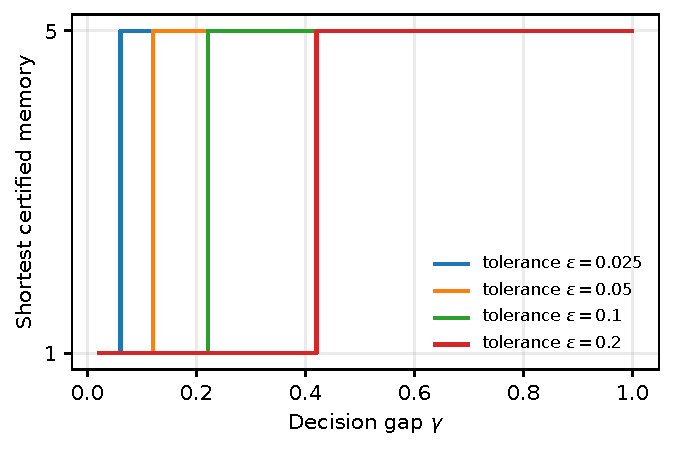
\includegraphics[width=\columnwidth]{../figures/soft_relevance.pdf}
  \caption{Population tolerance phase transition at horizon five.  An
  insufficient suffix has ambiguity \(\gamma/2\), so memory one is certified
  exactly when \(\gamma\leq2\epsilon\).}
  \label{fig:soft-supp}
\end{figure}

\begin{figure*}[t]
  \centering
  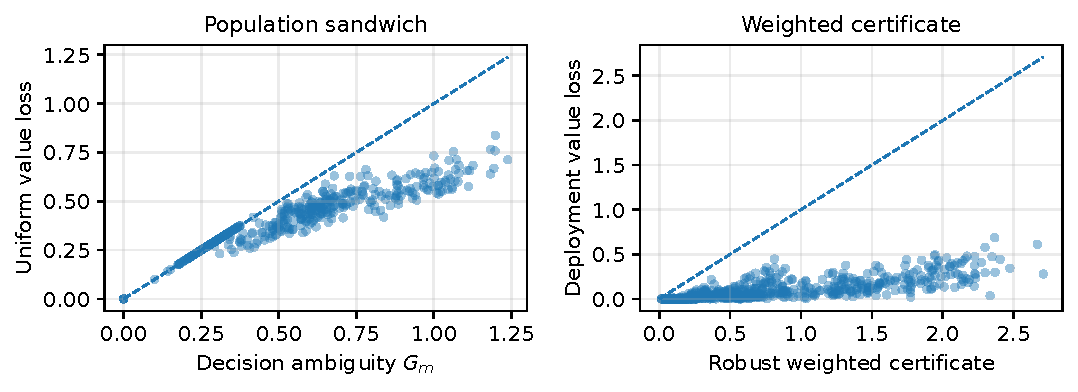
\includegraphics[width=0.94\textwidth]{../figures/random_stress.pdf}
  \caption{\textbf{Random history-MDP stress test.}  Left: the realized
  uniform value loss of the population minimax policy lies below \(G_m\).
  Right: the realized deployment loss of the robust weighted policy lies below its weighted certificate.
  Dashed lines denote equality.  The suite contains 700 memory
  configurations from 200 random history MDPs.}
  \label{fig:random-supp}
\end{figure*}

The random generator uses binary observations and actions.  Initial
observations and action-conditional next observations are sampled from
Dirichlet\((1,1)\), and each state-action mean reward is sampled from
Beta\((2,2)\).  Full action--observation histories remain distinct states, so
short suffixes induce random aliasing.  We use horizons three and four, 100
seeds per horizon, and synthetic \(Q^*\) interval half-width \(w=0.05\).
Across all 700 memory configurations, there are no failures of uniform
monotonicity, either side of the population sandwich, the robust certificate,
the \(2Hw\) inflation bound, the weighted population certificate, or the
weighted robust certificate.  The exact one-sided 95\% binomial upper bound on
the violation probability after observing zero failures is
\(1-0.05^{1/700}=0.427\%\).  Among configurations with nonzero realized
loss, the median relative slack of the uniform population upper bound is
24.6\%, with 90th percentile 65.5\%.

\begin{table*}[t]
\centering
\small
\begin{tabular}{p{0.16\textwidth}p{0.76\textwidth}}
\toprule
Experiment & Complete grid and repetitions \\
\midrule
Population separation & Tasks: delayed cue and predictive nuisance; horizons
\(\{2,3,4,5,6,8\}\); all candidate memories; balanced cue; gap one. \\
Soft relevance & Horizon five; 50 equally spaced gaps in \([0.02,1]\);
\(\epsilon\in\{0.025,0.05,0.1,0.2\}\). \\
Uniform calibration & Horizon four; \(p\in\{0.05,0.1,0.2,0.5\}\);
\(n\in\{50,100,200,500,1000,2000,5000,10000\}\); gap 0.5;
\(\epsilon=0.1\); \(\delta=0.05\); 50 seeds per point (1,600 datasets). \\
Coverage--gap scaling & Horizon two;
\(p\in\{0.05,0.1,0.2,0.5\}\);
\(\gamma\in\{0.2,0.3,0.5\}\); eight sample sizes from 100 to 20,000;
\(\epsilon=\gamma/4\); \(\delta=0.05\); 30 seeds (2,880 datasets). \\
Weighted certificate & Gap 0.4, \(\epsilon=0.1\).  Population:
20 logarithmically spaced values of \(p\) from 0.01 to 0.5.  Finite sample:
\(p\in\{0.05,0.1,0.2,0.5\}\),
\(n\in\{1000,2500,5000,10000,25000,50000\}\), 15 seeds;
\(\delta=0.05\) split equally between \(Q\) and occupancy events
(360 datasets). \\
Random stress & Horizons \(\{3,4\}\); 100 seeds per horizon; every memory;
interval half-width 0.05 (200 MDPs and 700 configurations). \\
\bottomrule
\end{tabular}
\caption{All grids used in the reported experiments.  No result-dependent
hyperparameter search is performed.}
\label{tab:grids}
\end{table*}

\section{Computational Reproducibility}

All stochastic scripts construct seeds deterministically from the displayed
grid indices and expose the number of repetitions as a command-line argument.
For the tabular trajectory datasets, episodes are simulated in vectorized
stage batches and reduced to state--action counts, Bernoulli reward sums, and
transition counts.  This retains exact episode sampling while keeping the
largest sweep lightweight.
The reported artifacts were regenerated on Debian GNU/Linux 13 using five
AMD EPYC 9V74 vCPUs and 5.9 GiB RAM.  The software
stack was Python 3.13.5, NumPy 2.3.5, SciPy 1.17.0, pandas 2.2.3, Matplotlib
3.10.8, and pytest 9.0.2; continuous integration independently runs Python
3.11.  No GPU is used.  The repository includes raw CSVs, generated figures,
16 theorem-driven tests, and a single command that rebuilds all results and
both manuscripts.

The experimental metrics are certificate validity, simultaneous interval
coverage, false short-memory certification, correct-memory certification,
selected memory, realized value loss, and certificate slack.  These metrics
were chosen to test the finite-sample statements directly rather than to claim
benchmark dominance.  Recovery and certification rates are reported over
independent seeds; for the zero-violation randomized test we additionally
report an exact one-sided binomial bound.  Significance tests for pairwise
algorithm improvements are not used because the paper makes no such
performance-comparison claim.

\bibliography{references}
\end{document}
